%Fiquemos com Deus e Nossa Senhora!
%Sao Jose de Cupertino rogai por nos!!
%Honra teu pai e tua mae!
% ### Uses XeLaTeX ### %
% ### Needs beamer-master ### %
\documentclass[aspectratio=169]{beamer} %. Aspect Ratio 16:9

\usetheme{AI2} % beamerthemeSprace.sty
\usepackage[portuguese]{babel}
\usepackage[utf8]{inputenc}
\usepackage[T1]{fontenc}
\usepackage{ragged2e,gensymb}

\DeclareMathOperator*{\argmin}{arg\,min}
\DeclareMathOperator*{\argmax}{arg\,max}
\DeclareMathOperator{\sign}{sgn}

% DATA FOR FOOTER
\date{2021}
\title{- Modelo de Mistura de Gaussianas}
\author{João Paulo Papa}
\institute{Advanced Institute for Artificial Intelligence (AI2)}

\begin{document}
% ####################################
% FIRST SLIDE 						:: \SliTit{This is the Title of the Talk}{A. B. Name}{Sprace}
% SUB-TITLE SLIDE 					:: \SliSubTit{<title>}{<explanation}
% SUB-SUB-TITLE SLIDE				:: \SliSubSubTit{<title>}{<explanation}
% SLIDE WITH TITLE 					:: \SliT{Title}{Content}
% SLIDE NO TITLE 						:: \Sli{Content} 
% SLIDE DOUBLE COLUMN WITH TITLE 	:: \SliDT{Title}{First Column}{Second Column}
% SLIDE DOUBLE COLUMN NO TITLE 		:: \SliD{First Column}{Second Column}
% SLIDE ADVANCED WITH TITLE 			:: \SliAdvT{Title}{Content}
% SLIDE ADVANCED NO TITLE 			:: \SliAdv{Content}
% SLIDE ADVANCED DOUBLE WITH TITLE 	:: \SliAdvDT{Title}{First Column}{Second Column}
% SLIDE ADVANCED DOUBLE NO TITLE 	:: \SliAdvD{First Column}{Second Column}
% SLIDE BLACK						:: \Black{ <Content> }
% SLIDE WHITE						:: \White{ <Content> }
% ITEMIZATION 						:: \begin{itemize}  \iOn{First} \iTw {Second} \iTh{Third} \end{itemize}
% COMMENT TEXT				 		:: \note{<comment>}
% SECTION 							:: \secx{Section} | \secxx{Sub-Section}
% BOLD SPRACE COLOR				:: \bfs{<text>}
% TABLE OF CONTENT					:: \tocitem{<title>}{<content>}
% LEFT ALIGN EQUATION				:: \begin{flalign*}  & <equation> &   \end{flalign*}
% CENTER ALIGN EQUATION	S			:: \begin{gather*} <equations>  \end{gather*}
% SLASH								:: \slashed{<>}
% BAR								:: \barr{<letter>} instead of \bar{<letter>}
% THEREFORE						:: use \portanto (larger and bold}
% 2 or 3 MATH SYMBOLS				:: \overset{<up>}{<down>} &  \underset{<below>}{\overset{<above>}{<middle>}}  
% INSERT TEXT IN FORMULA			:: \ins{<text>}
% EXERCISE							:: \exe{<exercise #>}{<exercise text>}
% SUGGESTED READING BOX			:: \sug{<references>}
% CITATION							:: \cittex{<citation>}
% CITATION DOUBLE COLUMN 			:: \cittexD{<citation>}
% TEXT POSITION						:: \texpos{<Xcm>}{<Ycm>}{<text>} origin = center of slide : x right | y down
% REFERENCE AT BOTTOM  S/D SLIDE		:: \refbotS{<reference>} \refbotD{<reference>}
% HIDDEN SLIDE						:: \hid
% COLOR BOX 						:: \blu{blue} + \red{rec} + \yel{yellow} + \gre{green} + \bege{beige}
% FRAME 							:: \fra{sprace} \frab{blue} \frar{red} + \fray{yellow} + \frag{green}		
% FIGURE 							:: \img{X}{Y}{<scale>}{Figure.png} 
% FIGURE							:: \includegraphics[scale=<scale>]{Figures/.png}
% FIGURE DOUBLE SLIDE NO TITLE		::  \img{-4}{0.5}{<scale>}{Figure.png} % Image 1st half
%									::  \img{4}{0.5}{<scale>}{Figure.png} % Image 2nd half
% FIGURE DOUBLE SLIDE WITH TITLE		::  \img{-4}{0}{<scale>}{Figure.png} % Image 1st half
%									::  \img{4}{0}{<scale>}{Figure.png} % Image 2nd half
% INCLUDING SWF (Flash)				:: \usepackage{media9} and \includemedia >> USE ACROBAT <<
%%%%%%%%%%%%%%%%%%%%%%%%%%%%%%%%%%%%%%%%%%%%%%%%%%
% ###############################################################################
% FIRST SLIDE
\SliTit{{\LARGE Modelo de Mistura de Gaussianas}}{Advanced Institute for Artificial Intelligence -- AI2}{https://advancedinstitute.ai}
%%%%%%%%%%%%%%%%%%%%%%%%%%%%%%%%%%%%%%%%%%%%%%%%%%
% ###############################################################################
% SLIDE SUB-TITLE
%\SliSubTit{Sub-Title}{Description}{}
%%%%%%%%%%%%%%%%%%%%%%%%%%%%%%%%%%%%%%%%%%%%%%%%%%
% ###############################################################################
%\SliSubSubTit{Sub-Sub-Title}{Description}
 %%%%%%%%%%%%%%%%%%%%%%%%%%%%%%%%%%%%%%%%%%%%%%%%%%


\SliT{Introdução}{

\justifying Modelo de Misturas de Gaussianas, do inglês \emph{Gaussian Mixture Models} - GMMs, é uma técnica de \textbf{aprendizado não supervisionado} vista como uma generalização do $k$-Médias. Ao invés de estimarmos os centroides de cada agrupamento, tentamos estimar também a forma e proporção de cada Gaussiana que compõe a mistura.\vspace{-.4cm}\newline

\justifying \underline{Definição do problema:} seja ${\cal X}=\{\boldsymbol{x}_1,\boldsymbol{x}_2,\ldots,\boldsymbol{x}_m\}$ um conjunto de dados tal que $\boldsymbol{x}_i\in\mathbb{R}^n$. Assumimos que as amostras são independentes e identicamente distribuídas (i.i.d.) a partir de uma função de densidade de probabilidade $p(\boldsymbol{x}_i)$, $\boldsymbol{x}_i\in{\cal X}$. Assumimos, também, que $p(\boldsymbol{x}_i)$ é uma \textbf{mistura finita} de $K$ componentes, ou seja:
\vspace{-0.1cm}
\begin{equation}
	p(\boldsymbol{x}_i|\boldsymbol{\theta}) = \sum_{k=1}^Kw_kp(\boldsymbol{x}_i|\theta_k),
\end{equation}
em que $\boldsymbol{\theta}=\{(w_1,\theta_1),(w_2,\theta_2),\ldots,(w_K,\theta_K)\}$, $\theta_k = (\boldsymbol{\mu}_k,\boldsymbol{\Sigma}_k)$ corresponde aos parâmetros relativos à Gaussiana $k$ e $\sum_{k=1}^Kw_k=1$.
}

\Sli{
As componentes $p(\boldsymbol{x}_i|\theta_k)$ são densidades Gaussianas multivariadas dadas por:

\begin{equation}
	p(\boldsymbol{x}_i|\theta_k) = \frac{1}{(2\pi)^{m_k/2}|\Sigma_k|^{1/2}}\exp\left\{-\frac{1}{2}(\boldsymbol{x}_i-\boldsymbol{\mu}_k)^T\boldsymbol{\Sigma}_k^{-1}(\boldsymbol{x}_i-\boldsymbol{\mu}_k)\right\},
\end{equation}
em que $m_k$ corresponde ao número de amostras que pertencem à Gaussiana $k$ tal que $m=m_1+m_2+\ldots+m_K$. No caso, os pesos $w_k$ representam a probabilidade que uma amostra $\boldsymbol{x}_i\in{\cal X}$ selecionada aleatoriamente tenha sigo gerada pela componente $k$. Vejamos o exemplo de uma mistura 1D com $K=3$.

\begin{center}
	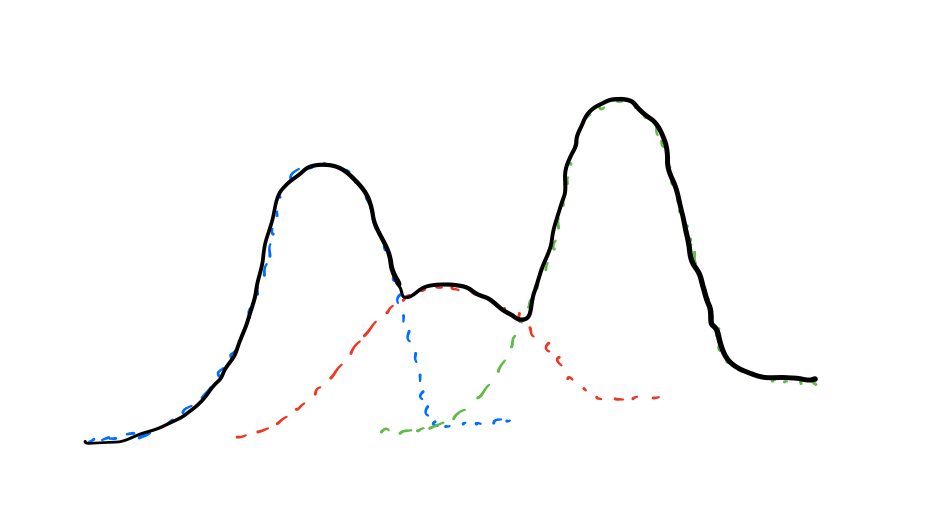
\includegraphics[scale=0.18]{./figs/GMM_Fig1.png}
\end{center}
}

\SliT{Treinamento}{

\justifying Como não temos os rótulos, devemos utilizar alguma informação adicional para estimar $\boldsymbol{\theta} = \{\theta_1,\theta_2,\ldots,\theta_K\}$. Para tal tarefa, podemos empregar o conhecido algoritmo E-M (\emph{Expectation-Maximization}), o qual segue a mesma ideia da abordagem de máxima verossimilhança.\newline

\justifying A falta do rótulo dos dados caracteriza um \textbf{problema estatístico incompleto}, fazendo com que utilizemos as chamadas \textbf{variáveis latentes}, isto é, variáveis que \textbf{não são observadas}. Note que no caso do classificador Bayesiano temos o conjunto de rótulos, ou seja, observamos essas variáveis.
}

\Sli{
\justifying Seja ${\cal Z}=\{z_1,z_2,\ldots,z_m\}$ um conjunto de variáveis latentes tal que $z_i\in\mathbb{N}$ e que cada uma delas está relacionada com uma amostra do conjunto de treinamento ${\cal X}$. Dado o conjunto de parâmetros $\boldsymbol{\theta}$, temos que a função de verossimilhança é dada por:

\begin{equation}
	L(\boldsymbol{\theta}|{\cal X},{\cal Z}) = p({\cal X},{\cal Z}|\boldsymbol{\theta}),
\end{equation}
\justifying em que $p({\cal X},{\cal Z}|\boldsymbol{\theta})$ corresponde à densidade conjunta de ${\cal X}$ e ${\cal Z}$. Ademais, o estimador de máxima verossimilhança do vetor de parâmetros $\boldsymbol{\theta}$ é dado, então, pela \textbf{maximização da verossimilhança marginal} (só temos acesso ao ${\cal X}$) dos dados observados, ou seja:

\begin{equation}
	L(\boldsymbol{\theta}|{\cal X}) = p({\cal X}|\boldsymbol{\theta}) = \int p({\cal X},{\cal Z}|\boldsymbol{\theta})\mathrm{d}{\cal Z}.
\end{equation}
A formulação acima corresponde à calcular a integral da probabilidade conjunta em ${\cal Z}$.
}

\Sli{
\justifying No entanto, não temos como calcular essa integral manualmente, pois não temos conhecido de ${\cal Z}$. No entanto, o algoritmo E-M é um estimador iterativo para a verossimilhança marginal. Ele funciona por meio da aplicação sucessiva de dois passos:

\begin{enumerate}
	\item \emph{Expectation} (E): calcula o valor esperado do logaritmo da verossimilhança com relação à distribuição condicional de ${\cal Z}$ dado ${\cal X}$ utilizando a estimativa atual dos parâmetros $\boldsymbol{\theta}$:
	\begin{equation}
		Q(\boldsymbol{\theta}|\boldsymbol{\theta}^{(t)}) = \mathbb{E}_{{\cal Z}|{\cal X},\boldsymbol{\theta}^{(t)}}[\log L(\boldsymbol{\theta}|{\cal X},{\cal Z})],
	\end{equation}
	em que $Q$ denota uma "quantidade".
	\item \emph{Maximization} (M): encontra os parâmetros que maximizam essa quantidade $Q$:
	\begin{equation}
		\boldsymbol{\theta}^{(t+1)} = \argmax_{\boldsymbol{\theta}}Q(\boldsymbol{\theta}|\boldsymbol{\theta}^{(t)}).
	\end{equation}
\end{enumerate}
De maneira geral, a ideia do algoritmo E-M é executar os passos 1 e 2 de maneira iterativa até que $|\boldsymbol{\theta}^{(t+1)}-\boldsymbol{\theta}^{(t)}|<\epsilon$. \textbf{A variável latente ${\cal Z}$ nos diz, basicamente, a pertinência de uma dada amostra $\boldsymbol{x}\in{\cal X}$ pertencer à um determinado agrupamento (classe).}
}

\Sli{
Basicamente, temos as seguintes informações acerca de nosso problema:

\begin{itemize}
	\item Observações em ${\cal X}$ podem ser discretas ou contínuas (ex: podem ser oriundas de distribuições Gaussianas).
	\item Variáveis latentes em ${\cal Z}$ são discretas (pseudo-rótulos).
	\item Os parâmetros em $\boldsymbol{\theta}$ são contínuos.
\end{itemize}
}

\Sli{
Basicamente, os passos do E-M são os seguintes:

\begin{enumerate}
	\item Inicializar o conjunto de parâmetros $\boldsymbol{\theta}$ de maneira aleatória.
	\begin{itemize}
		\item \underline{Passo E:} para cada amostra $\boldsymbol{x}_i\in{\cal X}$ associamos uma pontuação $\gamma_{ki}$ que denota a probabilidade dessa amostra pertencer ao agrupamento $k$, em que $\gamma\in\mathbb{R}^{K\times m}$.
		\item \underline{Passo M:} dadas as pontuações para todas as amostras, ajustamos $\boldsymbol{\theta}_k$ para cada Gaussiana (agrupamento) $k$ utilizando utilizando uma função de verossimilhança marginal (Equação 4).
	\end{itemize}
	\item Avaliamos a função do logaritmo da verossimilhança. Caso ela tenha estabilizado entre as iterações, podemos assumir que o método convergiu e interrompemos o processo treinamento.
\end{enumerate}
No entanto, uma maneira melhor de inicializar $\mu_k$ e $\Sigma_k$ é via algoritmo do $k$-Médias, em que $k=1,2,\ldots,K$. Já os pesos $w_k$ podem ser inicializados como $w_k = \frac{m_k}{m}$, em que $m_k$ corresponde ao número de amostras do agrupamento $k$.
}

\Sli{
Vamos às equações de atualização:

\begin{itemize}
	\item \underline{Passo E:} temos que as pontuações na iteração $t$ podem ser calculadas como segue:
	\begin{equation}
		\gamma^{(t)}_{ki} = \frac{w_kp(\boldsymbol{x}_i|\boldsymbol{\mu}_k,\boldsymbol{\Sigma}_k)}{\sum_{j=1}^Kw_jp(\boldsymbol{x}_i|\boldsymbol{\mu}_j,\boldsymbol{\Sigma}_j)}.
	\end{equation}
	A equação assim equivale ao preenchimento da matrix $\gamma$.
\end{itemize}
}

\Sli{
\begin{itemize}
	\item \underline{Passo M:} as seguintes equações são então utilizadas para atualizar os valores dos parâmetros:
\end{itemize}

\begin{equation}
	m_k = \sum_{i=1}^{m}\gamma^{(t)}_{ki},
\end{equation}

\begin{equation}
	\boldsymbol{\mu}_k^{(t+1)} = \frac{1}{m_k}\sum_{i=1}^{m_k}\gamma^{(t)}_{ki}\boldsymbol{x}_i,
\end{equation}

\begin{equation}
	\boldsymbol{\Sigma}_k^{(t+1)} =\frac{1}{m_k}\sum_{i=1}^{m_k}\gamma^{(t)}_{ki}(\boldsymbol{x}_i-\boldsymbol{\mu}_k)^T(\boldsymbol{x}_i-\boldsymbol{\mu}_k),
\end{equation}
e
\begin{equation}
	w_k^{(t+1)} = \frac{m_k}{m}.
\end{equation}
}

\Sli{
\justifying O logaritmo da verossimilhança é utilizado como critério de parada do algoritmo. Essa verossimilhança é uma medida de \textbf{confiança} que temos que os dados do conjunto de dados ${\cal X}$ são gerados pelos parâmetros estimados:

\begin{equation}
	\log p({\cal X}|\boldsymbol{\theta}) = \sum_{i=1}^{m}\log\left[\sum_{k=1}^Kw_kp(\boldsymbol{x}_i|\boldsymbol{\mu}_k,\boldsymbol{\Sigma}_k)\right].
\end{equation}
A equação acima deve ser calculada ao final de cada iteração do algoritmo E-M.
}

\end{document}